%
% File: chap_3.tex
% Author: Yuil Tripathee
%
\chapter{Requirements Elicitation}

\section{Elicitation Techniques}

To validate our hypothesis with market needs and quantize the requirements, we applied the elicitation techniques as follows.

\begin{itemize}
	\item Data Analysis
	\item Market Study
	\item Observation
	\item Prototyping and User Review
\end{itemize}

\section{Stakeholders}

Direct stakeholder acting in software include:

\begin{enumerate}
	\item Customers (Buyers and Sellers)
	\item Payment Gateway
\end{enumerate}

Here are the indirect stakeholder that have influence over software development, but not the direct actors in the system:

\begin{enumerate}
	\item Donation and Charity Campaigns
	\item Authorized Resellers
	\item Advertisement Companies
	\item Shipping providers
\end{enumerate}

\section{Use Case Analysis}

\begin{figure}[!h]
	\centering
	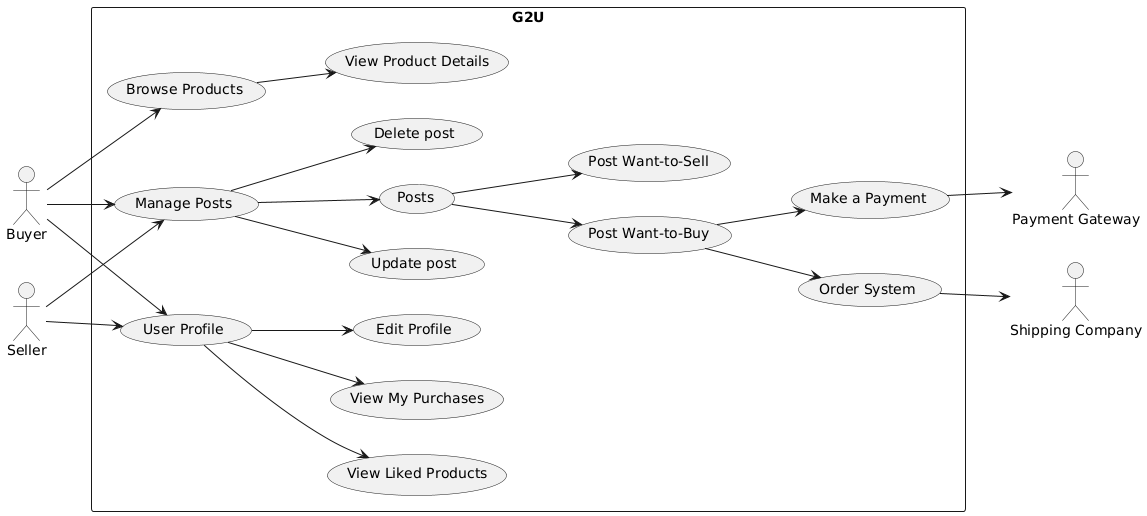
\includegraphics[width=1\textwidth]{chapters/ch-03/00_usecase.png} % Adjust width as needed
	\caption{Latest version of use case diagram after feedback driven iteration}
	\label{fig:usecase} % Label for referencing the figure
\end{figure}

%For software engineering observers, it is evident that use case diagram (in the Figure ~\ref{fig:usecase}) presented here is not in line with the data flow diagram. This is the result of agile practice. 

Initially, ~\ref{fig:usecase} had issues regarding the resemblance of DFD with the use case diagram. In the initial stages of engineering, we kept data flow analysis out of SDLC loop as it is redundant to sequence diagram (below). We can effectively model both system behavior, reaction (in terms of data changes and transfers) much effectively across our implementation team. Later to maintain the documentation, this work pattern was reverted and DFD diagram now is consistent to our use case diagram.

Upon final correction, we decided to incorporate data flow diagram as we modify our flow of application according to the user stories. Here, user stories are dictated by each individual use cases. Therefore, the data flow diagram which is created for the overall understanding of the system is maintained to be consistent with our changes in the use case diagram with the best of our abilities.

The use cases that are linked to preceding use case are well explained in the level 2 category of data flow diagram below. We attached it this way so that overall system is easily readable in the level 1 of DFD and finer details is based on conditions if the actor chose to access the particular small usecases (say Filter Products).

\section{System Analysis - Data Flow}

Figure ~\ref{fig:DFD0} and ~\ref{fig:DFD1} represents data flow diagram in level 0 and 1 respectively.

\begin{figure}[!h]
	\centering
	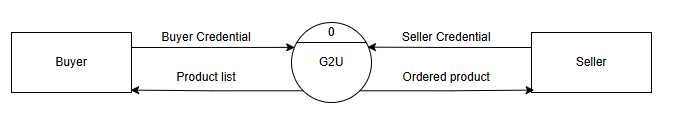
\includegraphics[width=0.75\textwidth]{chapters/ch-03/DFDL0.png} % Adjust width as needed
	\caption{Data Flow Diagram - Level 0}
	\label{fig:DFD0} % Label for referencing the figure
\end{figure}

\begin{figure}[!h]
	\centering
	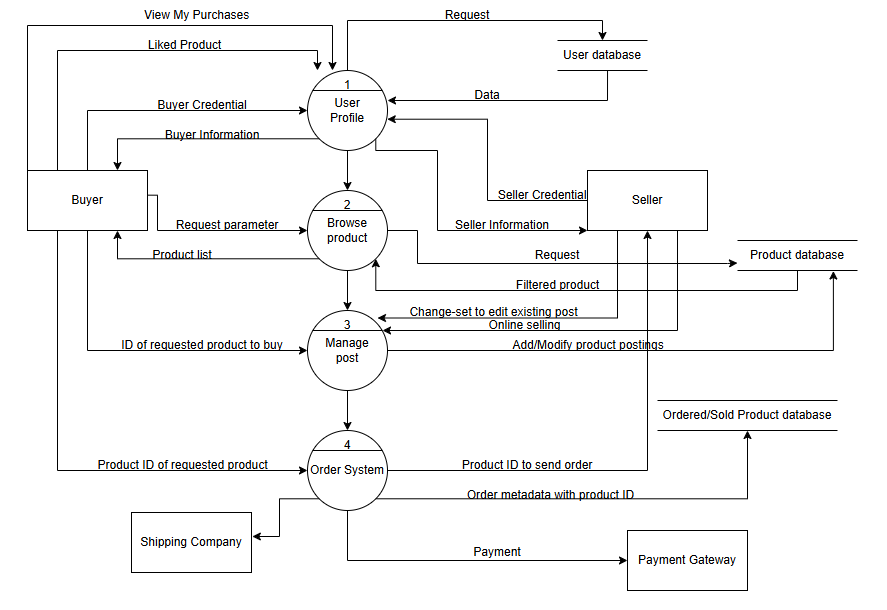
\includegraphics[width=0.8\textwidth]{chapters/ch-03/DFDL1.png} % Adjust width as needed
	\caption{Data Flow Diagram - Level 1}
	\label{fig:DFD1} % Label for referencing the figure
\end{figure}

And here comes the detailed DFD in level 2, this is separated into multiple parts starting from figure ~\ref{fig:DFD2}.

\begin{figure}[!h]
	\centering
	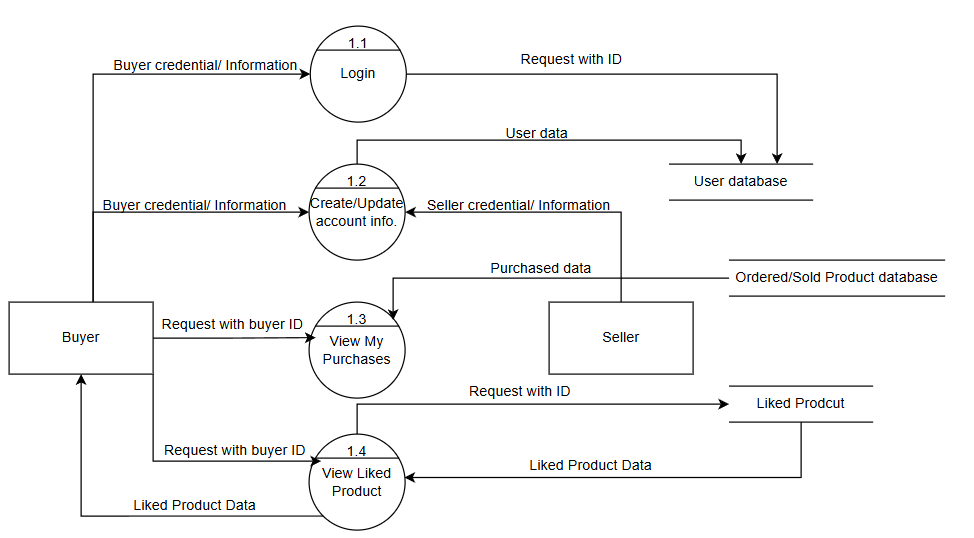
\includegraphics[width=1\textwidth]{chapters/ch-03/DFDL2_1.png} % Adjust width as needed
	\caption{Data Flow Diagram - Level 2 part 1}
	\label{fig:DFD2} % Label for referencing the figure
\end{figure}

\begin{figure}[!h]
	\centering
	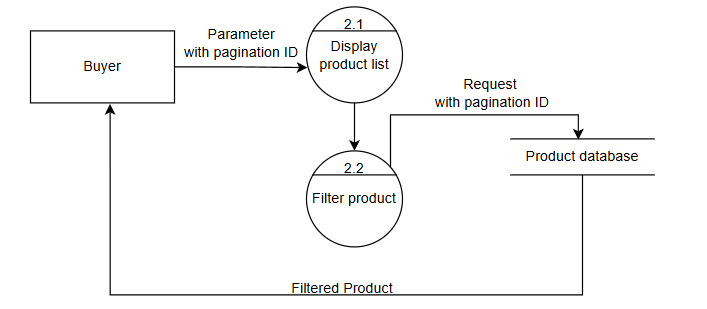
\includegraphics[width=1\textwidth]{chapters/ch-03/DFDL2_2.png} % Adjust width as needed
	\caption{Data Flow Diagram - Level 2 part 2}
	\label{fig:DFD2_2} % Label for referencing the figure
\end{figure}

\begin{figure}[!h]
	\centering
	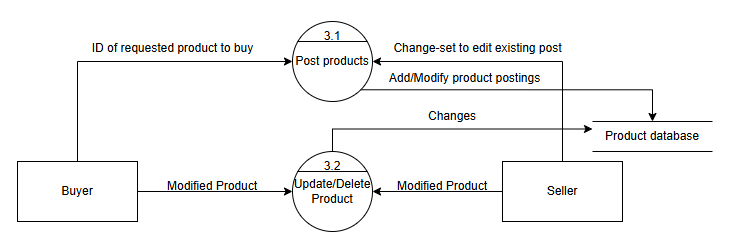
\includegraphics[width=1\textwidth]{chapters/ch-03/DFDL2_3.png} % Adjust width as needed
	\caption{Data Flow Diagram - Level 2 part 3}
	\label{fig:DFD2_3} % Label for referencing the figure
\end{figure}

\begin{figure}[!h]
	\centering
	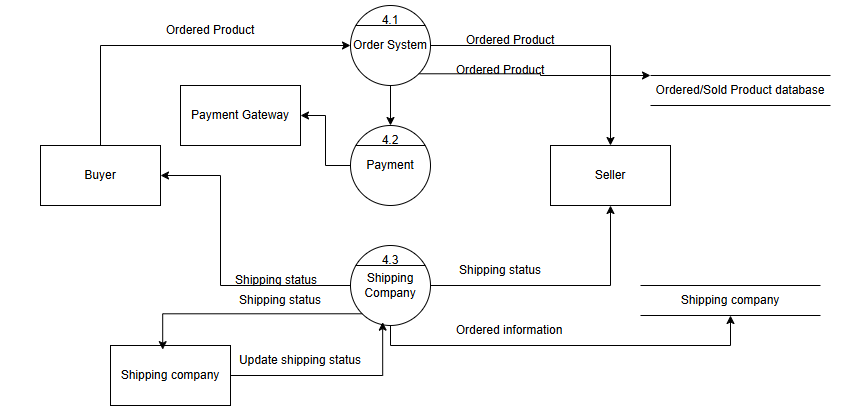
\includegraphics[width=1\textwidth]{chapters/ch-03/DFDL2_4.png} % Adjust width as needed
	\caption{Data Flow Diagram - Level 2 part 4}
	\label{fig:DFD2_4} % Label for referencing the figure
\end{figure}

\section{Functional Design}

Here are some functional requirements prior to user's evaluation and feedback resolution. This based on market validation of our brainstormed hypothesis.

\begin{enumerate}
	\item Internal escrow system to tackle scam issues.
	\item User management.
	\item Payment and shipping.
\end{enumerate}

During our application of Agile methodology, we can use these use case to track the progress based on user stories. For example, Browse Product can be a user story. Therefore, we can track the progress of certain specific elements from requirement to coding and document in this manner.

%\textit{TODO: Each functional requirements should have details and implementation in description list}

This is the tentative use case diagram (figure ~\ref{fig:usecase}) which evolved as a result of validating our hypothesis throughout continuous user feedback and CI/CD practice.

\section{Other Non-functional requirements}

\begin{description}
	\item[Scalability] 1000 concurrent users, with minimal architectural changes.
	\item[Availability] 99.5\% uptime (43.8 hours of annual downtime)
	\item[Security] Oath 2.0 with 256-bit encryption, implement VPC rules on database access.
	\item[Usability checker] 3 testing sessions with 5-10 users in MVP phase.
	\item[Performance] $< 200 ms$ for 50th percentile on server, $< 100 ms$ per query on database without performance degradation.
\end{description}

\subsection{Mandated constraints}

 The system must remain cost-effective during initial development and deployment, adhering to the constraints of a lean startup model. Expenses should prioritize scalability and maintainability, with a focus on minimizing fixed costs during the early stages. Therefore, incremented funding methodology allows us do financial checks over every incremental investment per feature addition or improvement.

\subsection{Regulatory compliance}

Briefly here are the regulatory issues we have encountered so far in the Thai business environment:

\begin{description}
	\item[ETA] ETA compiles data security requirements.
	\item[PDPA] safeguards user data.
	\item[Tax compliance] facilitate tax invoicing which is important for us and especially our B2B customers.
\end{description}

In the European side,

\begin{description}
	\item[GDPR] implements data protection rules especially in EU jurisdictions.
	\item[E-commerce directives] safeguards customer protection.
	\item[Fiscal obligations] to comply with local laws, including VAT collection and reporting.
\end{description}

\clearpage